
%%%%%%%%% MASTER -- compiles the 4 sections

\documentclass[11pt,letterpaper]{article}

%%%%%%%%%%%%%%%%%%%%%%%%%%%%%%%%%%%%%%%%%%%%%%%%%%%%%%%%%%%%%%%%%%%%%%%%%
\pagestyle{plain}                                                      %%
%%%%%%%%%% EXACT 1in MARGINS %%%%%%%                                   %%
\setlength{\textwidth}{6.5in}     %%                                   %%
\setlength{\oddsidemargin}{0in}   %% (It is recommended that you       %%
\setlength{\evensidemargin}{0in}  %%  not change these parameters,     %%
\setlength{\textheight}{8.5in}    %%  at the risk of having your       %%
\setlength{\topmargin}{0in}       %%  proposal dismissed on the basis  %%
\setlength{\headheight}{0in}      %%  of incorrect formatting!!!)      %%
\setlength{\headsep}{0in}         %%                                   %%
\setlength{\footskip}{.5in}       %%                                   %%
%%%%%%%%%%%%%%%%%%%%%%%%%%%%%%%%%%%%                                   %%
\newcommand{\required}[1]{\section*{\hfil #1\hfil}}                    %%
\renewcommand{\refname}{\hfil References Cited\hfil}                   %%
%\bibliographystyle{apsr}                                              %%
%%%%%%%%%%%%%%%%%%%%%%%%%%%%%%%%%%%%%%%%%%%%%%%%%%%%%%%%%%%%%%%%%%%%%%%%%

%PUT YOUR MACROS HERE

%\newcommand{\bm}[1]{\boldsymbol{#1}} %makes bold math symbols easier
\newcommand{\R}{\textsf{R}\space} %R in textsf font
\newcommand{\X}{\bm{\mathcal{X}}} %shorthand for iid
\renewcommand{\P}{\mathcal{P}}
\newcommand{\bt}{\pmb{\theta}}
\newcommand{\bl}{\pmb{\lambda}}
\newcommand{\bL}{\pmb{\Lambda}}
%\newcommand{\bG}{\pmb{\Gamma}}
\newcommand{\bh}{\pmb{\text{h}}}
\newcommand{\h}{\pmb{\text{h}}}
\usepackage{amsmath,amssymb}
\def\citeapos#1{\citeauthor{#1}'s (\citeyear{#1})}
\DeclareMathOperator*{\argmax}{arg\,max}

\usepackage{tikz} 
\usetikzlibrary{arrows,shapes,trees} 
\usepackage{color}
\usepackage{wrapfig}
\usepackage[english]{babel}
%\usepackage[table]{xcolor}
\usepackage{colortbl}
\usepackage{array}
\usepackage{graphicx}% Include figure files
\usepackage{algorithmic}
\usepackage{dcolumn}% Align table columns on decimal point
\usepackage{bm}% bold math

%\usepackage[sectionbib]{natbib}

%\includeonly{NSFsumm}

\begin{document}


%%%%%%%%% SUMMARY -- 1 page, third person
% e.g:  "The PI will prove" not "I will prove"

% big set-up, project description
\noindent {\bf \Large Project Summary} \vspace{.1cm}

\noindent The massive quantities of textual communications generated within most organizations constitutes a largely untapped source for insightful, real-time organizational analytics. From understanding external demands placed on organizations to summarizing the pressing intra-organizational players and issues, most salient developments are documented in digitized text. The content and context recorded in an organization's textual record can be leveraged to understand and improve an organization's performance. The basis of this project lies in two recent developments. First, recent research shows that the patterns and structure of communication, formalized as communication networks, are extremely important to effective organizational and individual problem-solving.  Second, many organizations, particularly government entities, have developed open textual input platforms in order to improve responsiveness to user (e.g., citizen, customer) needs. This project builds an analytical bridge between intra-organizational communication networks and streams of external input. Specifically, we will develop methods to parse and summarize the the contents of (1) input streams from external sources and (2) intra-organizational communication networks in the same topic-space, and understand the relationships between the external and internal domains.  \vspace{.25cm}

% Technical details, building credibility

\noindent {\bf Methodology:} We propose to study the ways in which government officials' communications with those outside of government are related to intra-governmental communications and government outputs. We will use US county government email archives acquired via public records requests and online data collection. We will design computational tools related to statistical topic modeling and network analysis that (1) identify topic-specific internal-external communication networks, (2) identify topic-specific internal communication networks and (3) learn the relationships between internal-external communications, intra-organizational communication networks and the contents of public policies.  The methods we develop will track the migration of topics to, within and from government. As such, we will characterize the democratic process at a fine-grained, content and context specific level.  The data we collect will permit extensive validation and innovative application of the algorithms developed. We will relate the core email data with additional publicly available data on county governments, including regulations/legislation and minutes from county legislatures. The proposed research will be conducted by an interdisciplinary team that brings expertise in tcomputational (Wallach) and social scientific (Desmarais) fields. \vspace{.25cm}

% Differentiating our approach from others (intellectual merit)

\noindent {\bf Intellectual Merit:} This project will offer important contributions to both computational and social sciences. In terms of computational approaches, we will enhance methods for the statistical analysis of text and network data. In particular, we will expand upon extant methods of textual network analysis in developing ways to learn (1) the topics that cut across network domains and (2) functions that characterize domain transfer of topics.  On the social science side, the methods we develop and data we collect will advance organizations' ability to connect streams of eternal input to their internal operations. Also, more directly, we will offer an unprecedented fine-grained assessment of government responsiveness at the local level in the US.  \vspace{.25cm}

% Broader Impa

\noindent {\bf Broader Impact:} This project will provide essential tools for organizations in providing timely and coherent responses to the demands of external constituencies. This holds potential to, e.g., improve the efficiency with which local governments manage public health needs, address environmental risks and establish revenue and spending policies. The contributions will be cross-disciplinary and will contribute to the broader scientific community. Also, we will provide an enormous data archive of government communication data to be tapped by other researchers.





\setcounter{page}{1}

%%%%%%%%% PROPOSAL -- 15 pages (including Prior NSF Support)

\section*{\Large Organizational Responsiveness to Open Outside Input:  A Modeling Approach based on Statistical Text and Network Analysis}


% From the NSF Grants Proposal Guide:
% "The Project Description should provide a clear statement of the work 
% to be undertaken and must include: objectives for the period of the proposed 
% work and expected significance; relation to longer-term goals of the PI's 
% project; and relation to the present state of knowledge in the field, 
% to work in progress by the PI under other support and to work in progress 
% elsewhere."

\section{Introduction}

Nearly every organization strives to respond in a timely and accurate manner to the needs and demands of some external constituency. Firms respond to customers, governments respond to citizens and educational institutions respond to students. The rapid advancement in communications technology over the last two decades has forever transformed the nature, volume and sources of input and feedback available to organizations. In addition, electronic communications have drastically improved the ability of organizations to document and communicate their internal developments. These complimentary developments have ushered into governance what has been termed 'we government' \cite{Linders2012}. Most elected officials can be directly contacted electronically through simple internet tools. Citizens can advertise and sign petitions on the web and attend internet 'town meetings' with their representatives. Regarding the internal activities of government, citizens can access electronic communications of their officials through public records requests, access meeting minutes on the web and, e.g., watch the floor activities of the US House of Representatives on HouseLive.gov. The emerging field of computational social science seeks to address the most pressing social scientific problems through the development of computational and statistical methods that are ideally tailored to the research task at hand. We propose to develop machine learning methods that are precisely tailored to modeling the {\em complete} input, deliberation, policy formation and implementation cycle documented in the electronic record surrounding an organization. In this collaborative project, which brings together researchers from computer science and political science, we will develop novel methods and apply them to the analysis of government responsiveness to public input across many US county and city governments.

\begin{wrapfigure}{r}{.5\textwidth}
\vspace{-.5cm}
\begin{center}
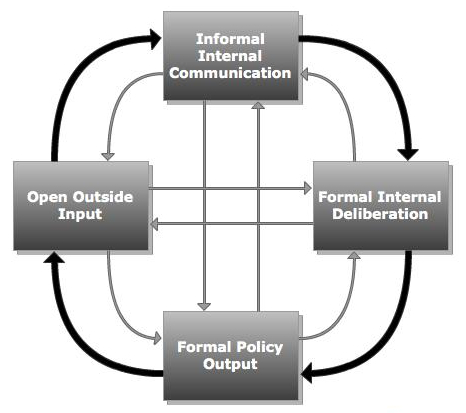
\includegraphics[scale=.525]{cycle.jpg}
\end{center}
\vspace{-.5cm}
\caption{Cycle of input, response and feedback. Black lines denote the normal IRF process and the gray lines represent alternative connections between domains. Direction of arrow indicates the temporal ordering of issue migration.}
\label{cycle}
\end{wrapfigure}

In this project we will develop and apply novel quantitative methods for identifying the cycle of input, response and feedback that leaves its fingerprint on the electronic communications record. We will focus on the nexus between government organizations and their constituents, but the methods we develop will be portable to other types of organizations. Government responsiveness to citizen input offers an ideal venue within which to model the relationship between streams of textual records embedded in different socio-organizational structural contexts (e.g., activist messages sent from independent citizens and regulations produced by a legislative body).  First, in democratic societies there is a common expectation that the government will respond to public demands. Second, the input mode on which we will focus-- direct email from the public to government officials -- is regularly central to government efforts to encourage direct input to the policy creation and implementation processes. Third, and perhaps of greatest practical importance, due to the scope of freedom of information laws in the US, we as researchers can access the public input and internal communications data associated with a multitude of government organizations.


We frame this project by associating different phases in the cycle of governance with four different types of textual streams and sociopolitical organizational contexts: public input (e.g., emails from citizens to government officials, informal internal communications (e.g., emails among officials), formal deliberations (e.g., legislative meeting minutes) and policy outputs (e.g., regulations, laws). We seek to understand these textual themes through the lens of multi-scale multi-corpora dynamic Bayesian latent variable models of textual content (i.e., topics \cite{Blei2003}) and organizational structural contexts (i.e., networks). We will develop (1) several domain-specific models of dynamic content and structure that are tailored to the unique characteristics of each corpus and (2) develop a flexible framework for constructing multi-corpora dynamic models that tie the individual domains together in a modular, extensible manner. The result will be an analytical approach that permits an organization to distill and investigate the dynamics of input, responsiveness and feedback through a common framework of statistical text analysis.  The methods we develop will offer answers regarding several pertinent questions about organizational management of outside input, e.g., is organizational attention to a topic proportional to its attention in outside input, how does an organization adapt to the rise of issues that are novel relative to its current foci, is responsiveness timely? 



Statistical topic models automatically infer groups of semantically-related words, known as topics, from word co-occurrence patterns within documents. A single topic is characterized by a discrete distribution over some vocabulary. Thus every word in the vocabulary is associated with every topic, albeit with varying probabilities. Given a corpus of documents, statistical topic models simultaneously infer the composition of the topics that best describe that corpus, as well a document-specific distribution over these set of topics for each document. In this way, every document is probabilistically associated with every topic.  \cite{Blei2010}. Statistical topic models provide a dually qualitative and quantitative inferential summary of textual corpora. They are qualitative in that the textual content of a corpus is maintained and quantitative in that the summary of the content is built through large-scale quantitative analysis of patterns in the content.  Since the seminal work on statistical topic models \cite{Blei2003}, the basic framework has been extended and adapted to focus on several aspects of textual corpora; including author-specific distributions over shared topics \cite{Steyvers2004}, dyadic (i.e., author-recipient) aspects of messages \cite{McCallum2005}, the underlying communication network \cite{Krafft2012}, and joint text-metadata models of documents \cite{Mimno2008}. Dynamic topic models provide an excellent framework within which to understand input to, output from and feedback to organizations that document their activities at various stages in a textual format . In the current project, we will undertake an ambitious set of extensions that integrate several of these extensions - jointly modeling separate streams of text that influence each other, are informed by rich meta-data, incorporate the underlying communication network, and characterize the over-time aspect of the text streams.


The benefit from connecting these innovations in statistical topic modeling is that we will leverage a medium common to each domain relevant to a cycle of organizational feedback and responsiveness - textual documentation to connect the domains as well as domain-specific metadata types. For example, in the case of governance, we will tie together the identities of citizens and groups providing outside input, the structure of communication networks underlying informal communications within government and voting coalition patterns within legislatures; all through the medium of the co-evolving, domain-specific text streams.


Figure \ref{cycle} Illustrates the cycle of organizational responsiveness that we intend to model through the guise of co-evolving textual streams. Considering the case of governance, substantial research exists that focuses on parts of this cycle. For example, a large body of research exists that documents recent developments in tools for citizens to provide precise, timely and voluminous input to government officials  \cite{Yildiz2007}. There is also a large body of research focusing on legislative adaptation to broad ideological trends among constituents \cite{Canes-Wrone2002}.  And, yet another literature that addresses the processes by which topics rise from informal awareness among officials and outside parties to the legislative agenda \cite{Baumgartner1993}. However, due to the historical inaccessibility of timely and common data modes related to each component of the governance cycle, little research has endeavored to connect all of the dots. We will provide such a complete picture, leveraging the common, available, and timely mode of text streams.


The disadvantage of analyzing relationships between domains in a separate, pairwise manner is that it is impossible to reconstruct a complete picture of the cycle of input, response and feedback relevant to an organization. For instance, in the example of governance, analysis of public input and any one government domain could provide a misleading account of government responsiveness. It may be the case that legislative meeting minutes document consideration of issues that are the subject of considerable public input. However, if final legislation is not responsive, it is not the case that democratic representation has run its complete course. And, initial research indicates that even the most advanced designs for encouraging direct input (i.e., e-petitions that trigger mandatory legislative attention) may end up having little to no policy influence \cite{Hough2012}.

The advantage of our approach will be that we will tap multi-channel input and response processes. This will allow us to identify fast-tracks and bottlenecks in the representation cycle. Identifying the dynamics of the entire system would inform those interested in providing outside input, those seeking to understand the overall responsiveness of an organization and those interested in affecting the organization's responsiveness.



\section{Open Outside Input and Governance}

At every level of government in the US, substantial resources have been dedicated to developing online platforms for citizen input to government. E-Rulemaking \cite{Coglianese2004} -- the process by which proposed regulations are posted to the internet and publicly deliberated on the web -- is the archetype of these efforts. US Federal agencies are required to post proposed rules to the website \texttt{regulations.gov} and provide a period for open commenting on the proposed regulation. Another mainstay of government operations in the information age is online tools to provide direct messages to public officials \cite{Balla2007}. Another recent example of open outside input was provided by President (elect) Obama in 2008. He established \texttt{Change.gov} during the transition to provide for direct citizen input to the administration's future priorities and activities \cite{Borins2009}. These developments mark a potential for rapid, massive and innovative ''citizen-sourcing'' of public policy - a form of democratic representation that is much more timely and rich than that realized through periodic elections and other forms of slower, less interactive input  \cite{Linders2012}.  

However, these developments raise several questions about the utility of these input and feedback modes. For example, do the actions of public officials and, ultimately, the content of public policy, reflect the inputs provided by citizens? Do public officials have the capacity to organize and summarize outside inputs? What characteristics of outside input predict the timely integration into public policy? All of these questions are critical to determining the value of these e-government or 'we-government' technologies.

We endeavor to answer these questions and more. Using fine-grained textual and contextual data on several stages of the input-response-feedback cycle, we will assess the dynamics of government responsiveness to open outside input on public policy. This will be made possible through the development of machine learning tools that connect multiple textual streams and a massive database of US county government records assembled through public records requests. This project is headed by a multidisciplinary team, which has already realized success in developing innovative machine learning tools to analyze novel databases on government communication networks. 


\section{Background: Public Records Data}

At the national, state and local levels, the US is the global leader in the scope and reliability of laws that guarantee access to information on government \cite{Halstuk2006}. The seminal legislation in this area is the federal Freedom of Information Act, which marks all information produced by executive agencies as public, unless the information meets at least one of seven criteria for exemption. Most US states have laws that mimic the federal legislation \cite{Braverman1980}, and most state laws subject localities (i.e, cities and counties) to public records archiving and disclosure requirements. North Carolina offers one of the broadest laws. For instance, email communications among local government officials are established by statute to be public record. 

Public record disclosure requirements establish a treasure trove for researchers. Many government organizations post significant text streams - from email communications with elected officials to meeting minutes - directly on websites. For categories of information not posted to the web, it is possible to make requests for the data. At all stages of the democratic process, local governments are required to archive textual records and provide them to the public upon request. This constitutes the primary advantage for focusing on government organizations in developing multi-stream models of the input-response-feedback cycle. 

\section{Project Team}

This project will be completed by a multidisciplinary team of computer scientist (Wallach) with background in developing machine learning methods for the statistical analysis of text and networks and a political scientist (Desmarais) with background in developing large scale statistical and network analytic models of political decision-making within US government institutions. The team is part of the UMass Amherst Computational Social Science Initiative and has already successfully completed and published pilot research that is highly relevant to the proposed project. This project will combine large-scale data collection, innovative methods development and social scientific analysis, resulting in the following deliverables.

\begin{itemize}
\item We will develop machine learning methods of statistical text analysis capable of characterizing the relationships between topics in separate dynamic corpora. In addition to extending dynamic topic models to multi-corpora relations, we will integrate corpora-specific-contextual data models. These methods will integrate several separate innovations in statistical topic modeling and provide a comprehensive textual and contextual data modeling framework that captures cross-domain migration of topics. 
\item We will provide a first-of-its kind, exhaustive micro-level assessment of the function of  democratic representation at the local level. The research we have on democratic responsiveness in the US focuses mainly on the federal or state governments. Our research will address local politics. Also, existing research on democratic representation addresses highly aggregated measures: e.g., showing that legislators from highly conservative districts vote, on average, more conservatively than those from more liberal districts. Our work will provide a fine-grained characterization of government responsiveness to the rise of public demands for action on specific public policy topics.
\end{itemize}



\section{Description of Pilot Research}

As an initial phase of research for this project, the team endeavored to leverage its expertise in the computational and social sciences, as well as the availability of rich data sources through the public record to address a challenge in the study of communication networks. A substantial body of research finds that the structure of a communication network has a substantial influence on the problem-solving abilities of the network as a whole and the performance of the individuals in the network \cite{Mason2012}. Moreover, recent research indicates that the topic or context of communication is important, meaning the measurement of a communication network should involve topic-of-discussion specificity \cite{Mason2008}. Thus, in order for an organization to diagnose and design its internal communication network, it must first be able to discern topic-specific communication networks.

Our pilot research addresses this problem \cite{Krafft2012}. Noting that email constitutes the cornerstone of most organizations' electronic communications, we focused on measuring and analyzing topic-specific communication networks using email archives. Using a public records request, we collected one months worth of in and out-box contents for all managerial-level employees of New Hanover County, North Carolina. We then developed a model that combined statistical topic modeling and the latent space model of social networks (a model that projects a network into a Euclidean space, within which actors who are close are more likely to connect than those who are far apart). Specifically, the model learns topic-specific latent spaces. This produces a coherent probabilistic generative model of corpus of messages annotated with sender-receiver information that permits intuitive visualization and analysis of the underlying topic-specific communication networks.

\section{Proposed Research}

We will advance machine learning methods for dynamic natural language processing and, using the methods we develop, provide a novel and insightful analysis of democratic responsiveness at the county level of government in the US. The tools we develop will be applicable to any level of government and other organization types. Our analysis of county governments will serve as a proof of concept and prototype for the use of our methods. Also, we will assemble a comprehensive multifaceted database of textual data on county governments that will prove useful to other researchers in natural language processing and the social sciences.

In the following sections we describe our approach to modeling the multi-domain cycle of input-response-feedback by first describing proposed datatypes and domain-specific model specifications then discussing our approach to tying the different domains together into a multi-component system.

\subsection{Modeling Outside Input}

To define a model for citizen input it is important to first identify the form of the data we will gather on citizen input. Via public records requests, we will collect all emails sent to county government officials by those outside of government. Though some government organizations have experimented with different electronic input modes, the email message is still the workhorse of direct advocacy {\bf cite}. We actually do not need to submit a separate request for this data, as they come with the in and out-boxes of government officials. 

We will model citizen input with a dynamic author-recipient topic model. The author-recipient topic model learns an overall topic model for the entire corpus as well as deviations for author-recipient pair \cite{McCallum2005}. We will consider both complete-email-address identifiers of 'authors' as well as email address domains as author signature - which may better handle input sent from the same organization but different people. The dynamic component will be handled with a logistic-normal model of topic dynamics \cite{Blei2006}. This approach will permit us to understand (1) the overall content of citizen input, (2) source-specific peculiarities in the content of input, (3) recipient-specific peculiarities of input content and (4) the over-time change in the content of input.

\subsection{Modeling Informal intra-governmental Communications}

The data for informal intra-governmental communications will also utilize the email data collected through public records requests. Since we will have all email for the officials, we will be able to model the complete communication network over time. In this phase of the model we will make the most explicit use of the team's pilot research. The model will constitute a dynamic topic-specific model of communication networks with the networks projected into Euclidean latent spaces. The topic dynamics will again be modeled using a logistic-normal specification. This characterization will permit us to understand how the content and network context of intra-governmental communications evolve.

Figure \ref{Figure:LatentSpace} illustrates the results from topic-partitioned communication network analysis. The dataset under analysis is a corpus of all emails among department managers from New Hanover County, North Carolina in the month of February, 2011. These are four selected topic-network-spaces. The word tokens listed at the top of the plots are the five most likely for the respective topic. Nodes are placed closer together in the inferred latent space if they are more likely to exchange emails on the respective topic. This modeling approach provides estimates that permit intuitive exploration of the structure of a communication network within a given topic.

\begin{figure*}[t]
\begin{minipage}[b]{0.5\linewidth}
\centering
\begin{tabular}{cc}
{\bf Public Signage} &
{\bf Broadcast Messages}\\
{\small change signs sign process ordinance}  &
{\small fw fyi bulletin summary week legislative} \\
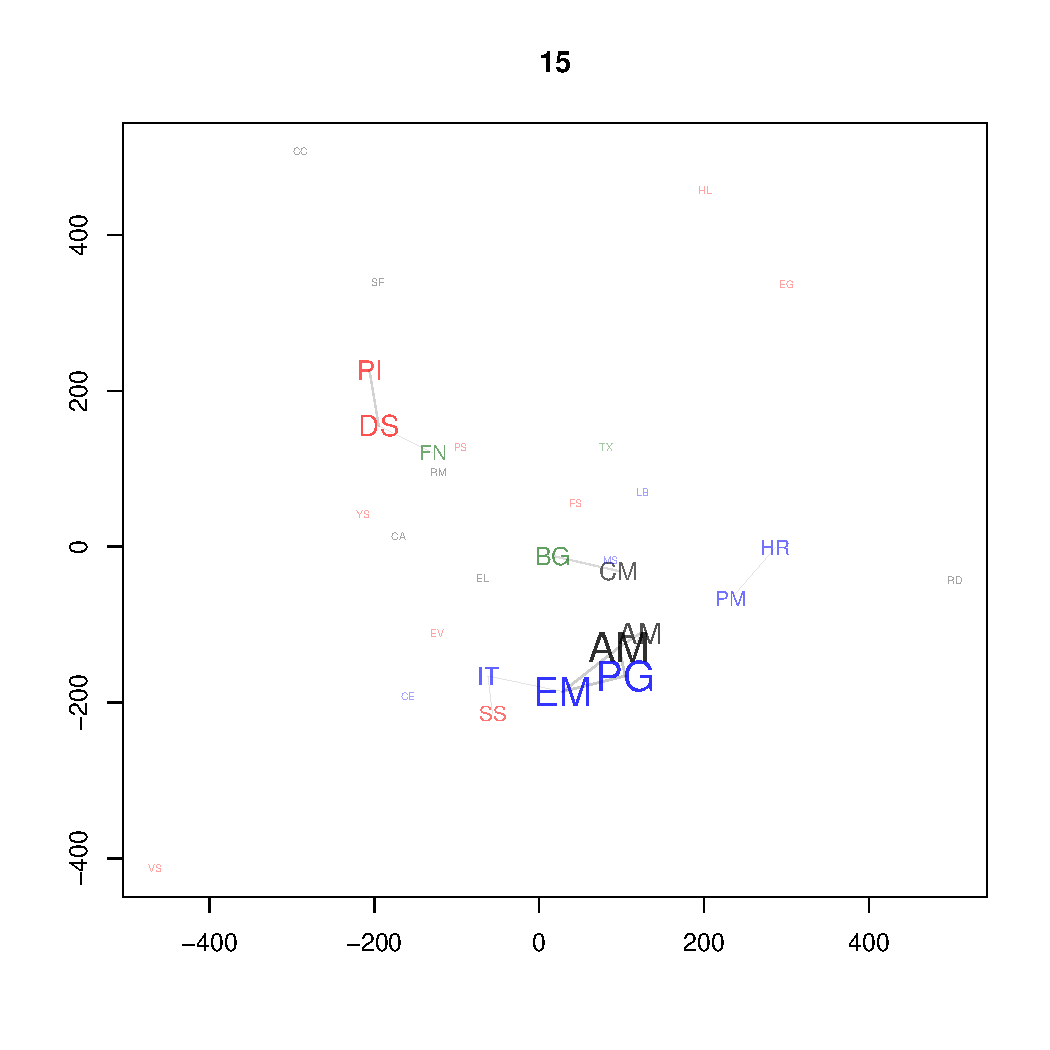
\includegraphics[scale=.29, trim=.4in .6in .4in .8in, clip=true]{latent_space_15} &
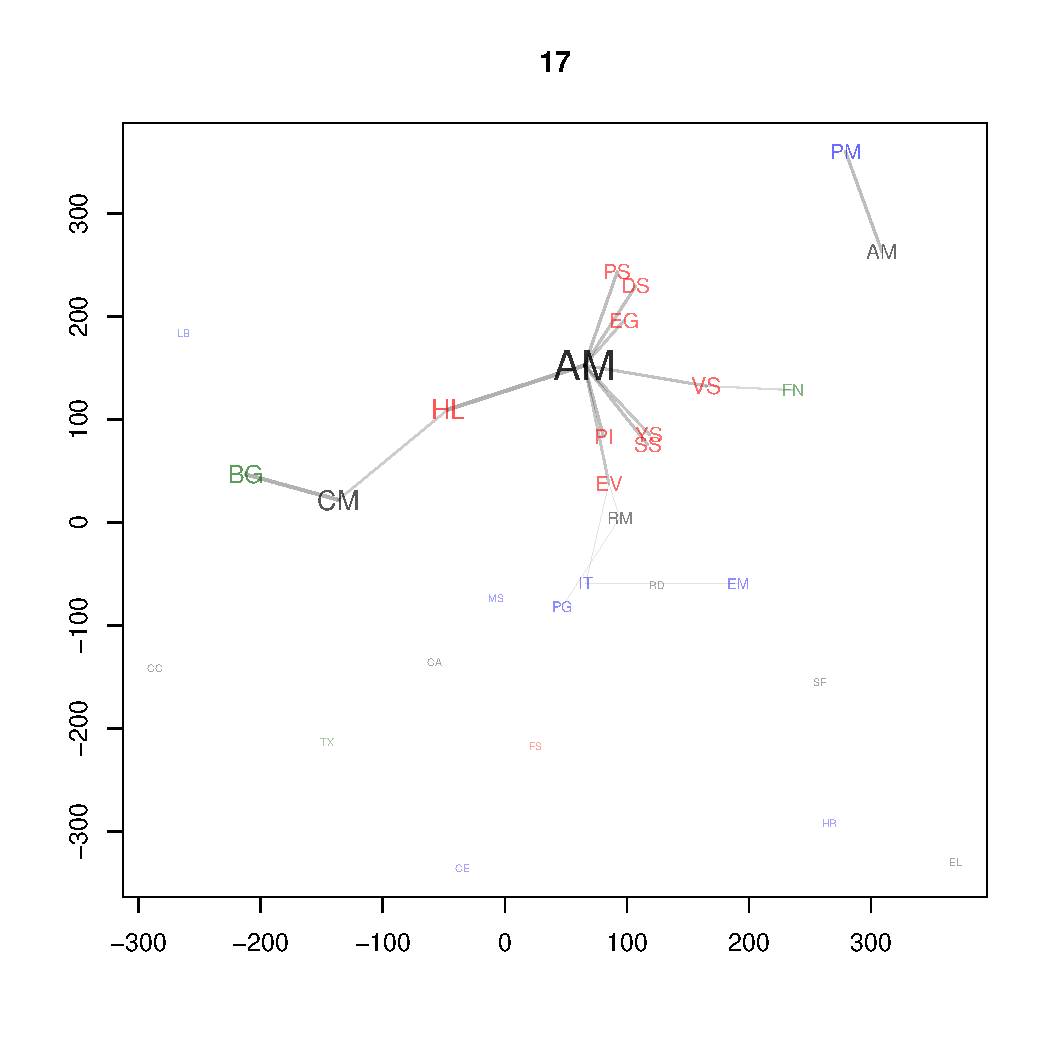
\includegraphics[scale=.29, trim=.4in .6in .4in .8in, clip=true]{latent_space_17} \\
{\bf Public Relations} &
{\bf Meeting Scheduling} \\
{\small city breakdown information give} &
{\small meeting march board agenda week} \\
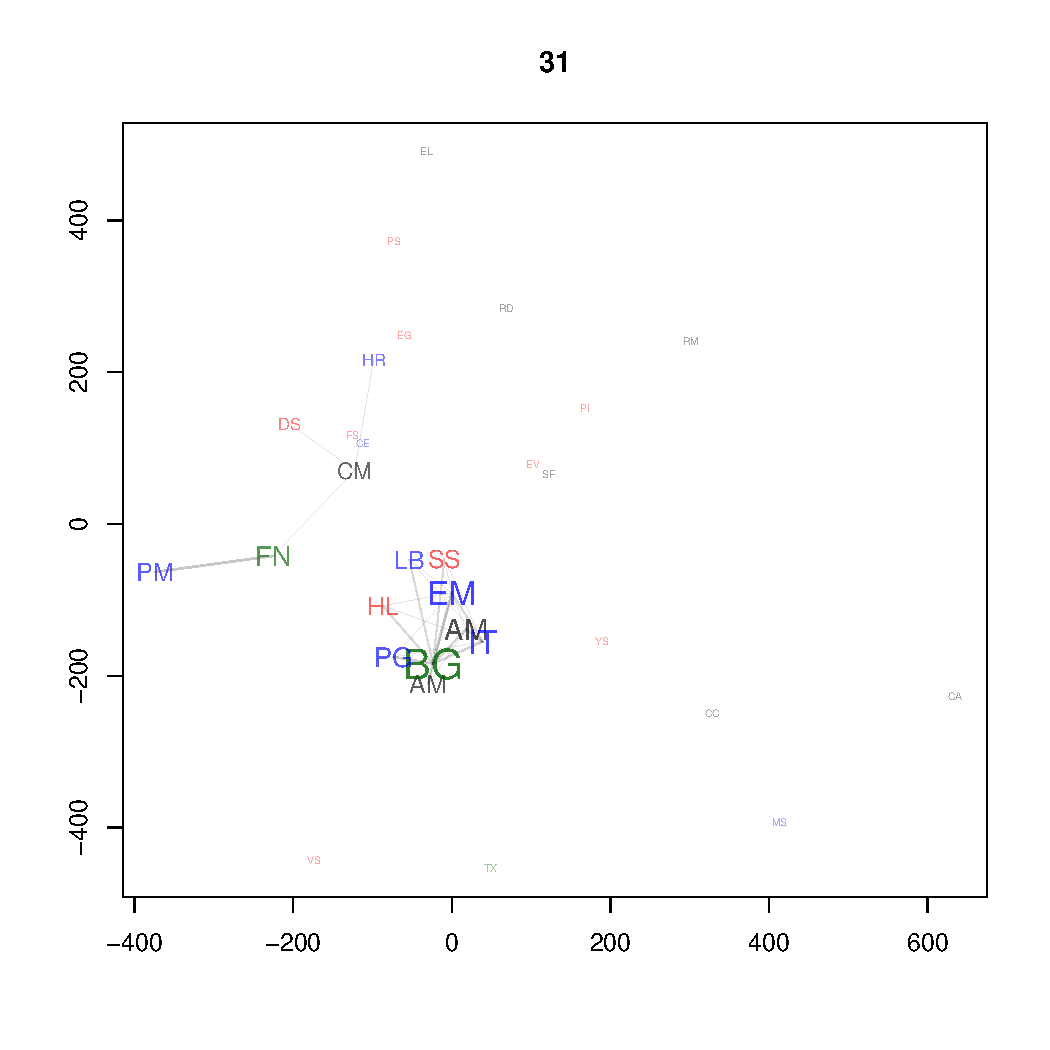
\includegraphics[scale=.29, trim=.4in .6in .4in .8in, clip=true]{latent_space_31} &
 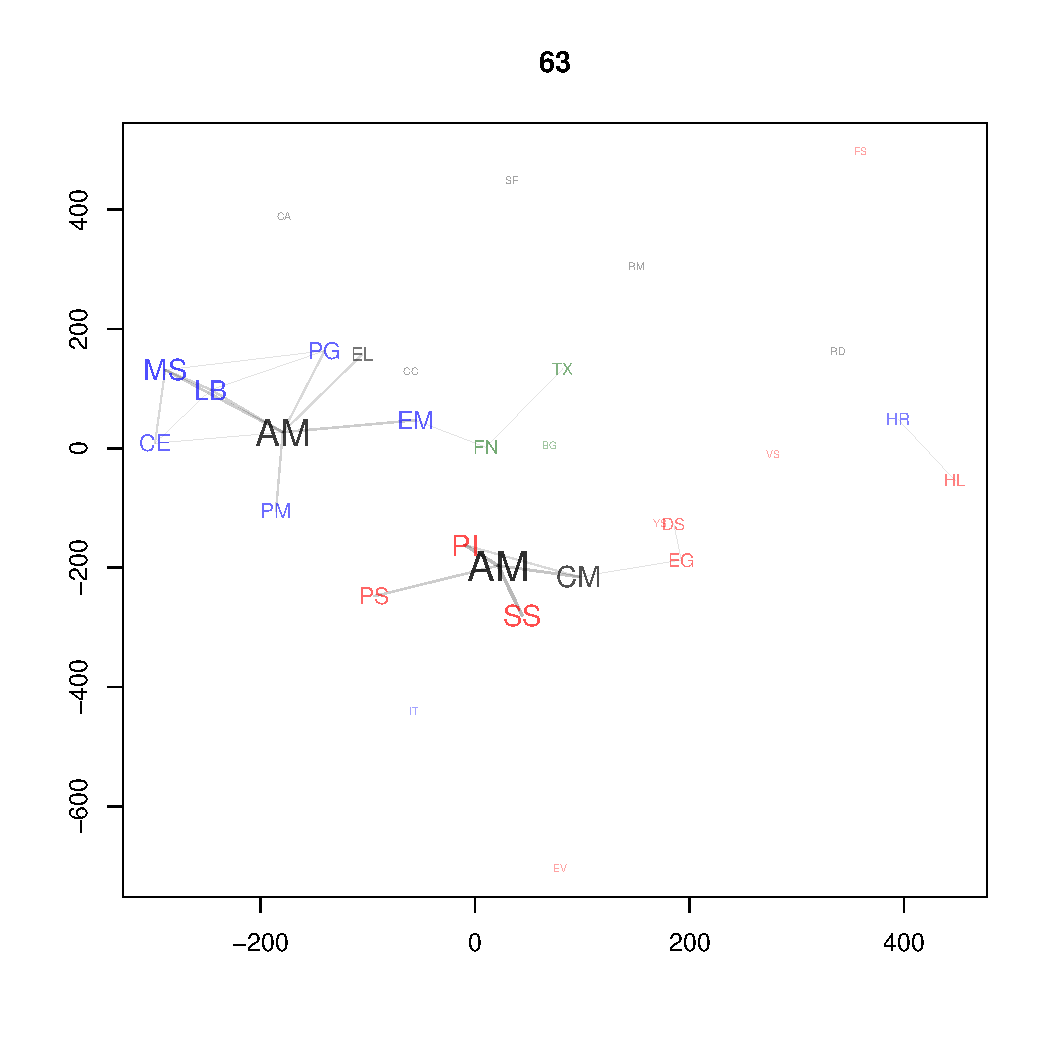
\includegraphics[scale=.29, trim=.4in .6in .4in .8in, clip=true]{latent_space_63} \\
\end{tabular}
\end{minipage}
\begin{minipage}{0.5\linewidth}
\hspace{3.25cm}\vspace{-0.4cm} 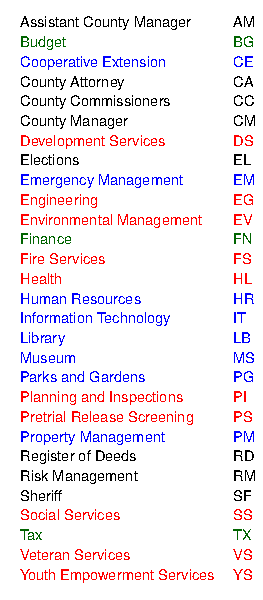
\includegraphics[scale=.85]{department_key}
\end{minipage}
\caption{Four topic-specific communication patterns inferred from the
  NHC email network. Each pattern is labeled with a human-selected
  name for the corresponding topic, along with that topic's most
  probable words in order of decreasing probability. The size of each
  manager's acronym in topic $t$'s pattern (given by $0.45 +
  1.25\,\sqrt{d^{(t)}_a \,/\, \max_a d^{(t)}_a}$, where $d^{(t)}_a$ is
  the degree of actor $a$ in that subnetwork) indicates how often that
  manager communicates about that topic.  Managers' acronyms are
  colored according to their respective division in the New
  Hanover County organizational chart. The acronym ``AM'' appears
  twice in all plots because there are two assistant county managers.}
\label{Figure:LatentSpace}
\end{figure*}

\subsection{Modeling Formal intra-governmental Communications}

Policy development that takes place at the county level occurs within county legislatures. Digitized archives of legislative meeting minutes are typically available on the web, but are certainly accessible via public records requests. If public records requests are fulfilled via paper delivery, we will use OCR to digitize the meeting minutes. This data will offer a window into whether issues that are being communicated to the government from outside actors and/or topics that arise through informal intra-governmental communications make their way to the legislative agenda. 

Our modeling approach with regard to legislative meeting minutes is informed by the political science literature on decision-making in legislatures. Most of this research focuses on the process of coalition-building in legislative processes \cite{Aldrich1995}. Since the vast majority of legislatures require majority support to establish policy, the primary task of a legislator is to lobby, placate and persuade his or her colleagues regarding proposed legislation. The coalition-building process gives rise to factionalism, which induces high positive association between the priorities of those in the same faction and high negative association between the priorities of those in different factions. 

We will implement an integrated version of the correlated topic model \cite{Blei2005} and author topic model \cite{Steyvers2004} and take advantage of the multiple-meeting structure of the data to assess the associations underlying the generation of meeting proceedings. Like the author topic model,  there will be a common set of topics discussed by all legislators at a given point in time, but proportional attention to topics will vary across legislators. The seminal correlated topic model embeds a correlation structure among topics. We will instead examine correlation between legislators' attention to topics. Specifically, we will parse each meeting into statements made by each county legislator. Then, we will fit a logistic-normal parameterization of the author-topic model that estimates a covariance matrix over legislators regarding their attention to topics in each meeting. This will capture the varying priorities among legislators and the correlations among them that arise through the legislative bargaining process.

\subsection{Modeling Legislative Output}

\begin{figure}[h]
\vspace{-.6cm}
\begin{center}
\begin{tabular}{m{2.5in}m{2.5in}} 
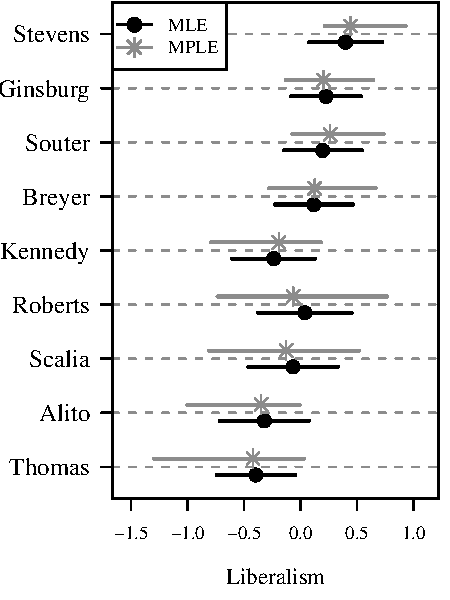
\includegraphics[scale=.65]{fixef} & 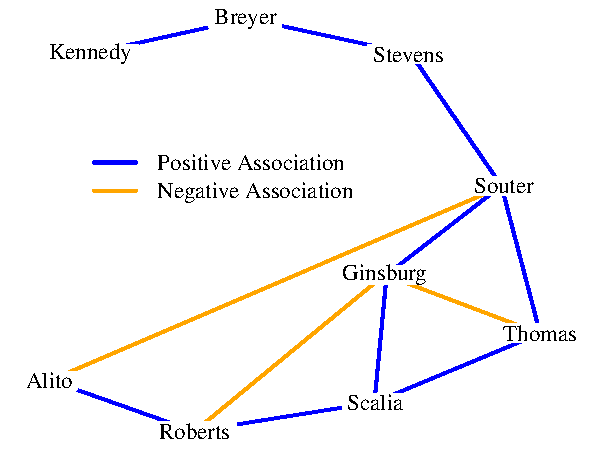
\includegraphics[scale=.75]{infnet}\\
(a) Estimates of Justices' Ideal Points & (b) Significant Associations Between Justices \\  
\end{tabular}
\end{center}
\vspace{-.3cm}
\caption{The bars in (a) span 95\% confidence intervals. In (b) an edge is drawn if the association parameter has the respective sign in at least  95\% of the bootstrap samples.}
\label{Figure:boltz}
\end{figure}


We will gather data on the statutes created by each county in order to examine implementation of topics that arise in the public, informal intra-governmental communications, and on the legislative agenda. These data are available on the web for most counties, and are certainly a matter of public record and would be available upon request. For some counties, it is straightforward to extract how legislators voted on a measure from the meeting minutes. For other counties, however, this is not as simple and may not be feasible. 

Regardless of whether we can extract votes on legislation, we will use a dynamic topic model with a logistic-normal autocorrelation structure  to model the content of legislation. If the votes are available, we will augment the dynamic topic model with a topic-specific network structure. The network will, however, take on a different form. The fully-visible Boltzmann Machine constitutes a probability model of jointly observed binary switches that is parameterized to model the tendency for each switch to be 'on' as well as the pairwise association between the states of each dyad of switches \cite{Gunawardana2008}. This can be used to model binary votes with voters akin to switches \cite{Desmarais2010}. This will allow us to jointly model the attention to topics in legislation as well as the associations among legislators' final votes on policy. Figure \ref{Figure:boltz} illustrates the results from applying a fully visible Boltzmann machine to vote data. Specifically, the data modeled are the votes of the nine justices in each US Supreme Court case from the 2007 and 2008 terms. The data are coded as 0 for a conservative vote and 1 for a liberal vote. Panel (a) gives the estimated tendencies of each justice to vote liberal and panel (b) depicts the strong positive and negative associations between justices. The Boltzmann machine offers a powerful approach to representing the individual and interactive tendencies among a group of decision-makers.


\subsection{Integrating Domain-Specific Models}

The overarching objective of our research is to model cross-domain relationships in topical attention throughout the input-response-feedback cycle underlying the democratic process. At the core of each domain-specific model is a statistical topic model of the domain-specific textual content. We seek to understand the relationships among the topic distributions, while also modeling the decision context in each domain. This will permit us to identify the points of tight coupling as well as breaking points in topic movement across domains.

The use of logistic-normal distributions in the construction of domain-specific topic distributions to model cross-domain relationships will constitute a highly flexible, illuminating and principled approach to tying the domains together in a complete cycle. We will derive models with a common set of topics across domains, but varying attention to topics in each domain. The attention to each topic will be given by a logistic transformation of Gaussian-distributed attention parameters. For each topic $t$, there will be four domain-specific attentiveness parameters. The four Gaussian attention parameters will be modeled as a vector autoregression \cite{Banbura2010}. This will permit topics to be related across domains. Thus, the attention level to a topic in each domain will be related to the attention level to a topic in every other domain, up to a selected number of periods into the past. 

A vector autoregression model is a classic linear regression model for time serial data. The estimated parameters of the vector autoregression model will be assessed in order to understand relationships across domains. This is a highly flexible framework for integrating domain-specific models. It works whenever a common set of topics is used to model the dynamic corpora across domains. Thus, this approach permits flexibility in tuning or possibly changing the form of the domain-specific models proposed above. Another major advantage of the vector autoregressive framework is that it constitutes an effective predictive forecasting model \cite{Banbura2010}. This would permit a forecast of, e.g., legislative attention to an issue in the future given current and past legislative, informal intra-governmental and outside input attention to an issue.

\subsection{Overall Project Outputs}

Each of the modeling phases described above constitutes a novel contribution to the literature on natural language processing. The four domain-specific models have not appeared in the literature in their proposed form. Each follows in the well established tradition of extending an existing NLP model to a dynamic model, adding an attribute/metadata component to a statistical topic model, or both. We expect to produce discrete papers related to each of these domain-specific models. 

The major machine learning contribution will be produced in the form of a paper describing our vector autoregressive logistic normal framework for constructing and learning topic models for cross-domain evolution in topic distributions. The framework will be motivated with the problem of modeling organizational responsiveness to outside input and illustrated through the combination of our domain-specific models to model the input-response-feedback cycle in local governments.

The major social scientific contributions will come in the form of several - likely two to four - journal articles. The domain-specific models will individually provide for important innovations in our understanding of government and local government processes. For instance, the analysis of email networks will permit us to assess whether government communication networks are structured to effectively solve problems. As a second example, the legislative meeting minute models will be useful in assessing whether political discussion is as factional at the local level as it is in the US Congress. The biggest contribution to political science offered by this project will be the analysis of the cross-domain relationships inferred using the vector autoregressive logistic-normal model. We will be able to speak in precise detail to a fundamental question of growing important to political scientists and practitioners alike -- how do governments respond to open outside input? 

Altogether, this proposed three year project will result in up to ten discrete papers -- all offering novel computational and/or social scientific contributions.

\section{Timeline and Division of Labor}

We propose to complete this research within a period of three years. The four major tasks will be (1) derivation and implementation of the NLP methods, (2) data collection and cleaning, (3) application of methods and assessment on empirical data, (4) social scientific analysis of results. We divide the project period into quarters and in Table 1, we provide a breakdown of the primary activities of the project, along with an assessment of when the tasks will be completed.


\begin{table}[h]
\caption{Schedule of Project Activities}
\begin{center}
\begin{tabular}{|l|l|l|l|}
\hline
{\bf Lead PI} & {\bf Activity} & {\bf Period} \\ \hline
Wallach & domain-specific model derivation   &   Q1-- Q3 \\ 
& and implementation &  \\ \hline
Desmarais & data collection (e.g., public records requests  & Q1-- Q3 \\
&  and web-scraping)  and organization & \\ \hline
Wallach & experimentation and assesment with county & Q4 -- Q7 \\
&  government data & \\ \hline
Desmarais & social scientific analysis  of & Q5 -- Q8 \\
& domain-specific results & \\ \hline
Wallach & development and application of integrated & Q8 -- Q12 \\
& vector autoregressive logistic normal model & \\ \hline
Desmarais & social scientific analysis of integrated & Q9 -- Q12 \\
& vector autoregressive logistic normal model & \\ \hline

\end{tabular}
\end{center}
\label{schedule}
\end{table}%



\section{Broader Impacts}

The proposed project will offer broad impacts that advance the core societal mission of the Information Integration and Informatics (III) program, directly enhance educational offerings at the University of Massachusetts and elsewhere and provide valuable interdisciplinary training opportunities related to an emerging area of research -- computational social science.

\subsection{Societal Mission}

The III program supports the development of computational tools and analytical approaches that enable the massive, diverse and complex streams of data to be efficiently utilized to produce scientific, technical and societal advances. Our proposed research addresses this mission, precisely. We will develop methods that enable organizations to assess their responsiveness to electronic open outside input using corpora of data that are already archived for other purposes (e.g., electronic messages, formal meeting records, distinct policy outputs). Also, on the more precise subject-matter of government responsiveness to outside input, we will assess the evidence for the effectiveness of 'we-government' style citizen contributions to the policymaking debate. In sum, this project will (1) offer computational tools that enhance the ability of organizations to remain responsiveness to outside input, (2) leverage large data archives already collected by countless organizations and (3) offer a critical assessment of a major new area of technological innovation for government. 

\subsection{Educational}

Both PIs are strongly committed to bringing their research into the classroom. PI Wallach regularly teaches a graduate seminar titled, 'Computational Social Science' in which state-of-the art innovations in computational social science are studied at-length. The results of the proposed project would certainly be integrated into the curriculum. PI Desmarais teaches graduate courses in network analysis at the University of Massachusetts and the University of Michigan (summer program). These courses integrate up-to-date methodological innovations in his research. The course material will be updated to reflect the contributions of the proposed project. PI Desmarais has also contributed to the NSF-supported Online Portal for Social Science Education in Methodology (OPOSSEM) - an open source online archive of methodological instructional materials. Instructional materials related to the current project would be posted to OPOSSEM.

\subsection{Training}

The proposed project will support a graduate student in computer science and one in political science at the University of Massachusetts, as well as several undergraduate research assistants.  The proposed research represents a genuinely interdisciplinary research program in the emerging field of computational social science. Long-term focused training for graduate students will provide valuable research experience and socialization on interdisciplinary projects - a growing focus of the scientific community. Undergraduate RAs will also gain valuable complimentary experiences. Computer science students will have the opportunity to work on technical problems that address highly important sociopolitical problems, and political science students will be directly exposed to the ways in which technical analysis and innovation can enhance knowledge of the public policy process.

\section{Results From Prior NSF Support}

% 5 pages or fewer of the 15 pages for entire description document.
% include results from NSF grants received in the past 5 years.
% if supported by more than one grant, choose the most relevant one
% for each grant, include: NSF award number, amount, dates of
% support, and publications resulting from this research.
% due to space limitations, it is often advisable to use citations rather
% than putting the titles of the publications in the body 
% of this section

% e.g.: "My prior grant, "Uses of Coffee in Mathematical Research" (DMS-0123456, 
% $100,000, 2005-2008), resulted in 3 papers [1],[2],[3], demonstrating..."

% if requesting postdoctoral research salary, a supplemental 1-page document
% called "Postdoc Mentoring Plan" will be required 


\setcounter{page}{1}

%%%%%%%%% REFERENCES -- no limit

% this should include only items referenced in the project description
% it is not a bibliography of related reading.

% Each reference must include the names of all authors (in the same
% sequence in which they appear in the publication), the article and 
% journal title, book title, volume number, page numbers, and year of 
% publication. If the document is available electronically, the website 
% address also should be identified

\bibliographystyle{ieeetr}
\bibliography{nsfbib}
\setcounter{page}{1}

\required{Data Management Plan}


\subsection*{A. Project Information}


\subsection*{B. General Data Management Plan Information }

\subsection*{C. Policies }

\subsection*{D. Legal Guidelines and Requirements }

\subsection*{E. Access, Sharing and Re-use of Data }



\subsection*{F. Data Standards and Capture }


\subsection*{G. Security, Storage, Management and Back-Up of Data }


\subsection*{H. Preservation, Review and Long-Term Management of Data }









\setcounter{page}{1}

%%%%%%%%% BIOGRAPHICAL SKETCH -- 2 pages


% Your Bio should be divided into the following sections
% (a) Professional Preparation (education):
% Undergrad, Major, Year
% Graduate, Major, Year
% Postdoc, Area, Years-Inclusive
% (b) Appointments:  most recent first.
% (c) Publications:  5 related to the proposal, and 5 "Other Significant Publications"
% (d) Synergistic Activities (math-enhancing activities that were not
% part of your main job description, like editorial boards and
% conference organizing - any Math-related volunteer work.
% these are often similar to Broader Impacts

% (e) Collaborators & Other Affiliations: (use the following sections)
% list in alphabetical order, and include current affiliations parenthetically
% Collaborators and Co-editors: past 48 months.  If none, write "none"
% Graduate Advisors and Postdoctoral sponsors: (your own, no matter how long ago)
% Thesis advisor and postgraduate scholar-sponsor:  those you have advised
% in the past 5 years.  
% Total number of graduate students advised: X (all time)
% Total number of postdoctoral scholars sponsored: Y (all time)

\required{Biographical Sketch: Bruce A. Desmarais}

\begin{enumerate}
\item[\textbf{(a)}] \textbf{Professional Preparation:}
\begin{enumerate}
\item[--] Eastern Connecticut State University, Economics and Public Policy, B.A.  (2002)
\item[--] University of North Carolina at Chapel Hill, Political Science, M.A.  (2008)
\item[--] University of North Carolina at Chapel Hill, Political Science, Ph.D. (2010)
\end{enumerate}
\textbf{\item[(b)] Appointments:}
\begin{enumerate}
\item[--] \emph{University of Massachusetts Amherst}
Assistant Professor, 2010 - Present 
\end{enumerate}

\textbf{\item[(c)] Publications}
\begin{enumerate}
\item[(i)] Publications Directly Related to the Proposed Project
\begin{enumerate}
\item[--] Peter Krafft, Juston Moore, Bruce Desmarais and Hanna Wallach. 2012. ``Topic-Partitioned Multinet-
work Embeddings.'' In \emph{Proceedings of the 26th Annual Conference on Neural Information Processing
Systems.}
\item[--] Cranmer, Skyler J. and Bruce A. Desmarais. 2011. ``Inferential Network Analysis with Exponential Random Graph Models.'' \emph{Political Analysis.} 19(1): 66-86.
\item[--] Desmarais, Bruce A. and Skyler J. Cranmer.  2012.``Statistical Inference for Valued-Edge Networks: The Generalized Exponential Random Graph Model" \emph{PLoS-ONE.} 7(1):e30136. 
\item[--] Desmarais, Bruce A. and Skyler J. Cranmer. 2012. ``Statistical Mechanics of Networks: Estimation and Uncertainty.'' \emph{Physica A} 391(4): 1865-1876.
\item[--] Desmarais, Bruce A. and Skyler J. Cranmer. 2012. ``Micro-Level Interpretation of Exponential  Random Graph Models with Application to Estuary Networks'' \emph{Policy Studies Journal.} 40(3): 402-434.

\end{enumerate}



\item[(iii)] Other Significant Publications
\begin{enumerate}
\item[--] Desmarais, Bruce A. 2012.``Lessons in Disguise: Multivariate Predictive Mistakes in Collective Choice Models.'' \emph{Public Choice}.  151(3--4): 719-737..
\item[--] Cranmer, Skyler J., Bruce A. Desmarais, and Elizabeth J. Menninga. 2012.  ``Complex Dependencies in the Alliance Network'' \emph{Conflict Management and  Peace Science} 23(3).
\item[--] Cranmer, Skyler J., Bruce A. Desmarais, and Justin H. Kirkland. 2012. ``Towards a Network Theory of Alliance Formation'' \emph{International Interactions}. 38(3): 295-324.
\item[--] Desmarais, Bruce A. and Skyler J. Cranmer. 2012. ``Micro-Level Interpretation of Exponential  Random Graph Models with Application to Estuary Networks'' \emph{Policy Studies Journal.} 40(3): 402-434.
\item[--] Desmarais, Bruce A. and Jeffrey J. Harden. 2012. ``Comparing Partial Likelihood and Robust Estimation Methods for the Cox Regression Model'' \emph{Political Analysis}. 20(1): 113-135.
\end{enumerate}
\end{enumerate}

\textbf{\item[(d)] Synergistic Activities}
\begin{enumerate}
\item[--] Co-organized an interdisciplinary speaker series in Computational Social Science at UMass Amherst (2010--Present) -- \texttt{http://cssi.umass.edu/seminars.html}.
\item[--] Editorial board member, {\em State Politics \& Policy Quarterly}, (2011--Present).
\item[--] Member of the fellowship committee for the 2012 Political Networks Conference.
\item[--] Participated in the founding and administration of the Triangle Political Methodology Group (2009--2010) -- \texttt{http://www.unc.edu/depts/polisci/methods/}. 
\end{enumerate}
\textbf{\item[(e)] Collaborators and other Affiliations}
\begin{enumerate}
\item[(i)] Collaborators
\begin{enumerate}
\item[--] Skyler Cranmer, University of North Carolina at Chapel Hill
\item[--] Jeffrey J. Harden, University of North Carolina at Chapel Hill
\item[--] Hanna Wallach, University of Massachusetts Amherst
\item[--] Brian Schaffner, University of Massachusetts Amherst
\item[--] Vincent Moscardelli, University of Connecticut
\item[--] Tobias Heinrich, Rice University
\item[--] Allison Freeman, Center for Community Capital (UNC Chapel Hill)
\item[--] Elizabeth Menninga, University of North Carolina Chapel Hill
\item[--] Justin Kirkland, University of North Carolina, Chapel Hill
\item[--] Rachel Shorey, University of Massachusetts Amherst
\item[--] Stuart Benjamin, Duke University
\item[--] Peter Krafft,  University of Massachusetts Amherst
\end{enumerate}

\item[(ii)] Graduate and Post-Doctoral Advisors
\begin{enumerate}
\item[--] Thomas Carsey, University of North Carolina Chapel Hill
\item[--] Skyler Cranmer, University of North Carolina Chapel Hill
\item[--] James Stimson, University of North Carolina Chapel Hill
\item[--] Kevin McGuire, University of North Carolina Chapel Hill
\item[--] Isaac Unah, University of North Carolina Chapel Hill
\end{enumerate}

\item[(ii)] Thesis Advisor
\begin{enumerate}
\item[--] Rachel Shorey, UMass Amherst Computer Science M.S. Student
\item[--] Peter Krafft, UMass Amherst Computer Science M.S. Student
\item[--] James Aaron, UMass Amherst Political Science Ph.D. Student
\item[--] Michael Kowal, UMass Amherst Political Science Ph.D. Student
\item[--] Manabu Nakashima, SUNY Albany Public Administration Ph.D. Student
\end{enumerate}
Total number of graduate students advised: 4

\end{enumerate}
\end{enumerate}


\setcounter{page}{1}
\required{Budget Justification}

\noindent \textbf{Senior Personnel}\\

\noindent \textbf{Other Personnel}\\


\noindent \textbf{Fringe Benefits}\\

\noindent \textbf{Travel}\\

\noindent \textbf{Other Direct Costs}\\


\noindent \textbf{Indirect Costs}\\

\newpage
\required{Facilities, Equipment and Other Resources}
\noindent \textbf{Laboratory}\\


\noindent \textbf{Clinical}\\

\noindent \textbf{Computing}\\


\noindent \textbf{Office}\\

\noindent \textbf{Major Equipment}\\

\noindent \textbf{Other Resources}\\

\noindent 






\end{document}
